\section[Introduction]{Introduction to version control}
\begin{frame}
	\frametitle{A basic example}
	\begin{columns}
		\begin{column}{0.5\textwidth}
		\begin{itemize}[<+->]
			\item Only one person can work on a file at a time
			\item Difficult to keep track on which file to use
			\item Difficult to compare the files
			\item Do you have back up?
			\item Probably more issues
		\end{itemize}
		\end{column}
		\begin{column}{0.5\textwidth}
			\begin{center}
				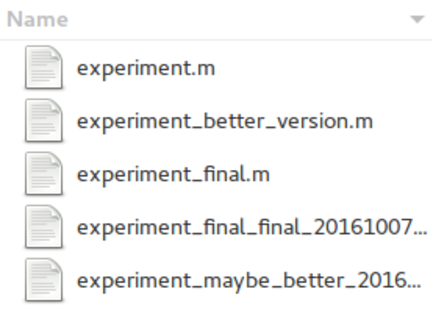
\includegraphics[width=\textwidth]{./pictures/simple.pdf}
			\end{center}
		\end{column}
	\end{columns}
\end{frame}

\begin{frame}
	\frametitle{Smarter way of doing it}
	\begin{columns}
		\begin{column}{0.5\textwidth}
			\begin{itemize}[<+->]
				\item Equivalent of storing your stuff on M
				\item Included in MAC
				\item Easy to set up
				\item Still difficult to collaborate
			\end{itemize}
		\end{column}
		\begin{column}{0.5\textwidth}
			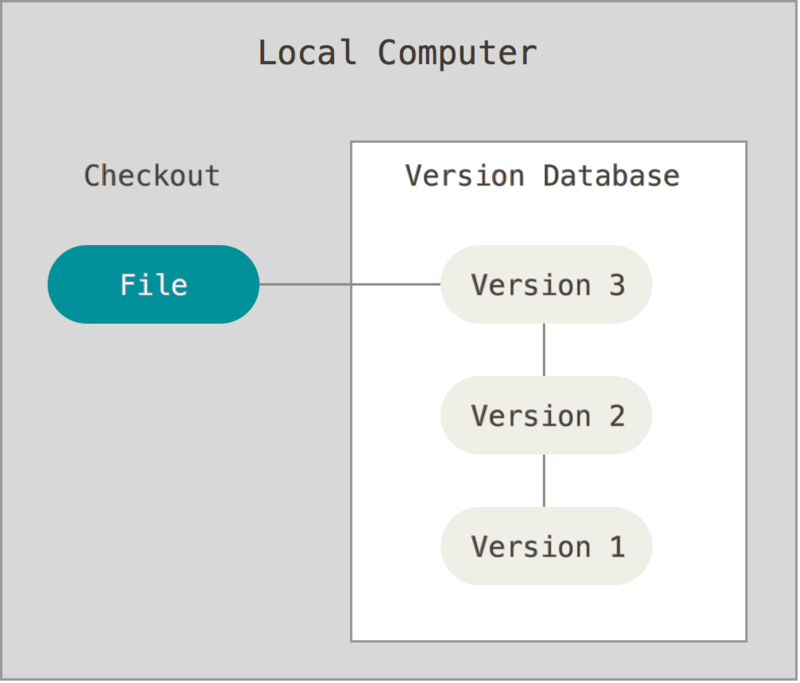
\includegraphics[width=\textwidth]{./pictures/local.png}
		\end{column}
	\end{columns}
\end{frame}

\begin{frame}
	\frametitle{Centralized version control}
	\begin{columns}
		\begin{column}{0.5\textwidth}
			\begin{itemize}[<+->]
				\item Examples:
						\begin{itemize}[<+->]
							\item CVS
							\item subversion
							\item perforce
						\end{itemize}
				\item Easy to collaborate
				\item Check out specific versions
				\item Single point of failure (N-0)
				\item If the server dies only checked out versions can be saved
			\end{itemize}
		\end{column}
		\begin{column}{0.5\textwidth}
			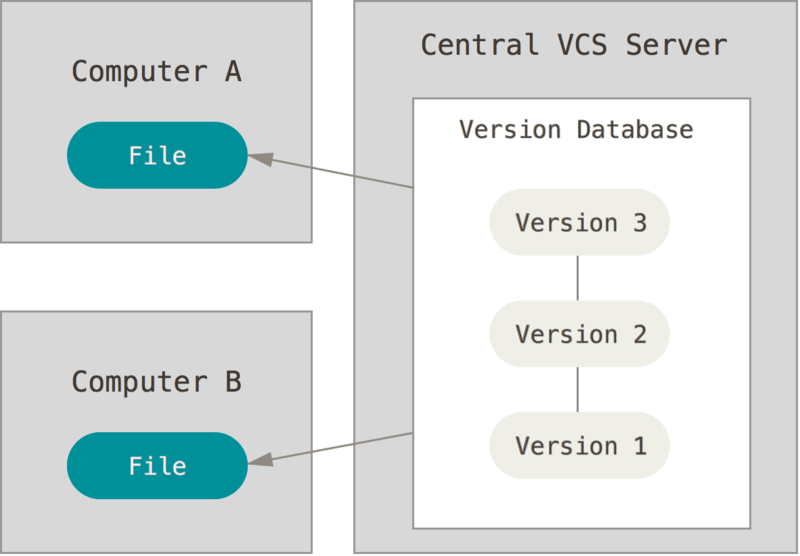
\includegraphics[width=\textwidth]{./pictures/centralized.png}
		\end{column}
	\end{columns}
\end{frame}

\begin{frame}
		\frametitle{Distsributed version control}
	\begin{columns}
		\begin{column}{0.5\textwidth}
			\begin{itemize}[<+->]
				\item Examples:
					\begin{itemize}[<+->]
						\item Git
						\item Mercurial
						\item Bazaar
						\item Darcs
					\end{itemize}
				\item Same advantages as centralized version control
				\item All users can reconstruct the project
				\item Easy to work against multiple servers
			\end{itemize}
		\end{column}
		\begin{column}{0.5\textwidth}
			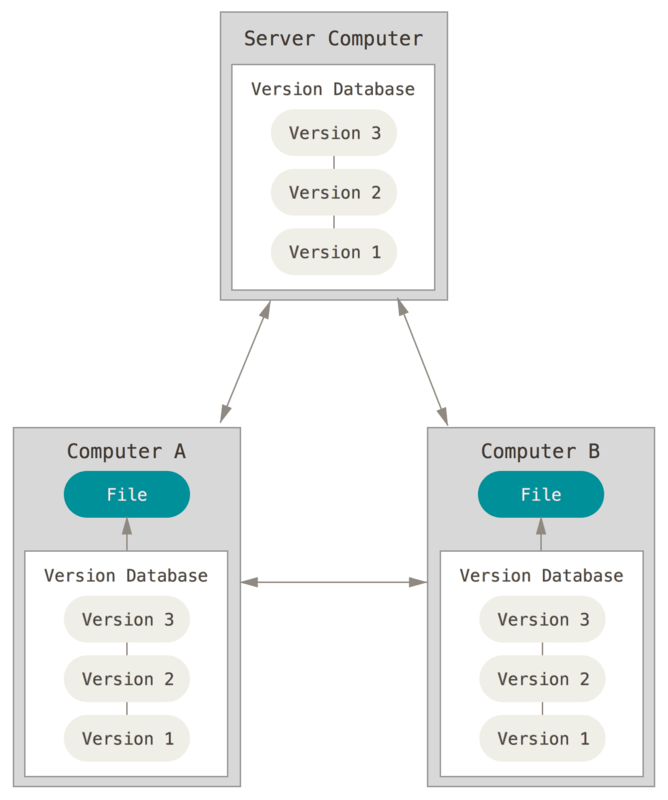
\includegraphics[width=\textwidth]{./pictures/distributed.png}
		\end{column}
	\end{columns}
\end{frame}

\begin{frame}[fragile]

	\frametitle{Should you use version control?}
	\begin{columns}
		\begin{column}{0.5\textwidth}
			\begin{itemize}[<+->]
				\item Do you write code?
					\begin{itemize}[<+->]
						\item If yes: use version control
					\end{itemize}
				\item Never copy code -\_-+
				\item Write functions and keep them version controlled
				\item Remember code is a virtual laboratory
				\item Versions can for instance be tagged with name of publication(reproducability for review)
			\end{itemize}
		\end{column}
		\begin{column}{0.5\textwidth}
			Dont do this:
			\lstinputlisting[style=Matlab-editor]{./examples/experiment.m}
		\end{column}
	\end{columns}

\end{frame}
